%LTeX: language=DE
\chapter{Vorbereitung}
	\begin{equation}
		U_{aus} = U_{Ref} \left( 1 + \frac{R_2}{R_1} \right) + I_{Adj} R_2
		\label{eq:output voltage}
	\end{equation}
	nach \(R_2\) umgestellt ergibt sich zu:
	\begin{equation}
		R_2 = \left( U_{aus} - U_{Ref} \right) \cdot \left( \frac{U_{Ref}}{R_1} + I_{Adj} \right)^{-1}
	\end{equation}

	Mit den aus dem Datenblatt zu entnehmenden Werten \cite{datasheet.LM317.TexasInstruments.2021} für \(U_{Ref} = \SI{1,25}{V}\), \(I_{Adj} = \SI{50\cdot 10^{-6}}{A}\) und \(R_1 = \SI{240}{\ohm}\) und einer vorgegebenen
	Ausgangsspannung \(U_{aus}\) von \SI{(5\pm0,1)}{V} ergibt sich \(R_2\) zu:
	\begin{align}
		R_2 &= \left( \SI{5}{V} - \SI{1,25}{V} \right) \cdot \left( \frac{\SI{1,25}{V}}{\SI{240}{\ohm}} + \SI{50\cdot10^{-6}}{A} \right)^{-1} \nonumber \\
			&\approx \SI{713,15}{\ohm} \nonumber
	\end{align}
	Unter Berücksichtigung allerdings, dass ein Wert von \SI{240}{\ohm} in der E-Reihe für Normwiderstände nicht aufzufinden ist,
	wird der nächstliegende Wert von \SI{270}{\ohm} gewählt. Hiermit ergibt sich für \(R_2\)
	\begin{align}
		R_2 &= \left( \SI{5}{V} - \SI{1,25}{V} \right) \cdot \left( \frac{\SI{1,25}{V}}{\SI{270}{\ohm}} + \SI{50\cdot10^{-6}}{A} \right)^{-1} \nonumber \\
			&\approx \SI{801,35}{\ohm}
	\end{align}
	Bei Vernachlässigung von \(I_{Adj}\) erhöht sich sein Wert auf \SI{810}{\ohm}. Beide jedoch liegen unter dem nächstliegenden
	Wert der E-Reihe von \SI{820}{\ohm}.\par
	Mit den gefundenen Bauteilwerten für die Widerstände \(R_1\) und \(R_2\) kann die zu erwartende Ausgangsspannung mit \cref{eq:output voltage}
	errechnet werden zu
	\begin{equation}
		U_{aus} = \SI{1,25}{V} \left( 1 + \frac{\SI{820}{\ohm}}{\SI{270}{\ohm}} \right) + \SI{50\cdot10^{-6}}{A} \cdot \SI{820}{\ohm} = \SI{5,09}{V}
		\label{eq:ausgangsspannung voila}
	\end{equation}
	Es konnte gezeigt werden, dass für diesen Fall der Beitrag durch den Justierstrom \(I_{Adj}\) sowohl für die Komponentenauswahl,
	als auch zur Betrachtung der Ausgangsspannung vernachlässigt werden kann.
	\begin{figure}[h]
		\centering
		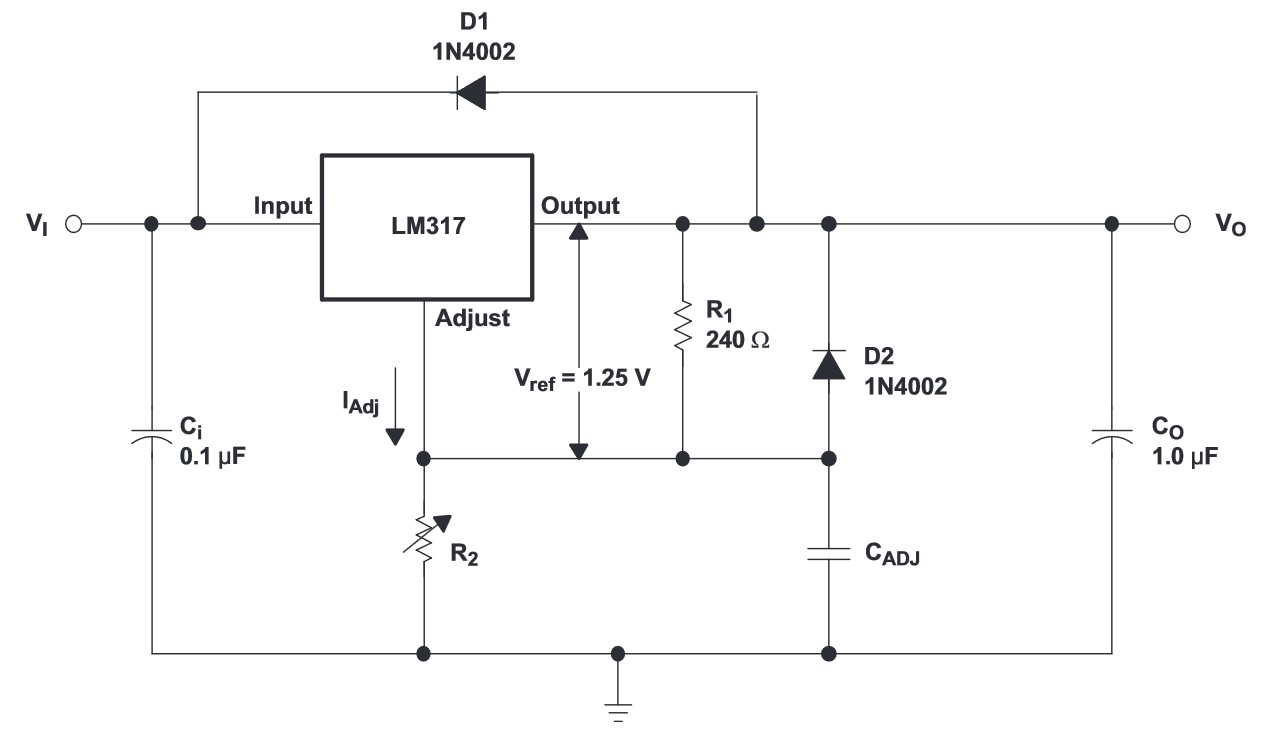
\includegraphics[width=.9\textwidth]{referenzen/typical_app_schem.jpg}
		\caption{Aus dem Datenblatt übernommenes Diagram eines typischen Anwendungsszenarios eines LM317 Linearreglers \cite{datasheet.LM317.TexasInstruments.2021}. Zentrale Elemente sind hier der Linearregler selbst, sowie
		die beiden Widerstände \(R_1\) und \(R_2\). \(R_2\) insbesondere dient hier zur justierung der Ausgangsspannung.}
		\label{fig:typical app sch}
	\end{figure}